\begin{LARGE}
\textbf{DETAILED CALCULATIONS}
\end{LARGE}
\\
\\


\section*{Detailed calculation of the gluon radiation of a quark}
\subsection*{$ |M_1|^2 $}

\begin{equation}
\begin{split}
|M_1|^2=(d-2)\:\frac{g_s^2  C_F }{(2k_1\cdot q_i)}
[\not{k_1} ][\not{q_k}]
\end{split}
\end{equation}

\begin{equation}
\begin{split}
&|M_1|^2=(d-2)\:\frac{g_s^2 \: C_F }{2y\: p_i \cdot Q}
[(\alpha_1 -y\beta_1(\frac{Q^2}{2p_i \cdot Q})) \not{p_i} + y\beta_1\not{Q} + \sqrt{y\alpha_1\beta_1}\not{n}_{\bot,1} ]\\
&[A_1\not{p_i} + A_2\not{Q} + \sqrt{1-y}\not{p_k}]
\end{split}
\end{equation}

\begin{equation}
\begin{split}
&|M_1|^2=(d-2)\:\frac{g_s^2 \: C_F }{2y\: p_i \cdot Q}
[(A_2(\alpha_1 -y\beta_1(\frac{Q^2}{2p_i \cdot Q}))+ A_1y\beta_1) {p_i}\cdot Q\\
&+(\alpha_1 -y\beta_1(\frac{Q^2}{2p_i \cdot Q}))\sqrt{1-y}p_i\cdot p_k+A_2 y\beta_1 Q^2+ \sqrt{1-y}\sqrt{y\alpha_1\beta_1}{n}_{\bot,1}\cdot p_k ]\\
\end{split}
\end{equation}

For the collinearity $ y \rightarrow 0 $ we'll get:

\begin{equation}
\begin{split}
&|M_1|^2=(d-2)\:\frac{g_s^2 \: C_F }{2y\: p_i \cdot Q}
[(A_2(\alpha_1 -y\beta_1(\frac{Q^2}{2p_i \cdot Q}))+ A_1y\beta_1) \not{p_i} \not{Q}\\
&+(\alpha_1 -y\beta_1(\frac{Q^2}{2p_i \cdot Q}))\sqrt{1-y}\not{p_i} \not{p_k}+A_2 y\beta_1 Q^2+ \sqrt{1-y}\sqrt{y\alpha_1\beta_1}\not{n}_{\bot,1} \not{p_k} ]\\
\end{split}
\end{equation}

\begin{equation}
\begin{split}
&|M_1|^2=(d-2)(1-\beta_1)\sqrt{1-y}\:\frac{g_s^2 \: C_F }{2y\: p_i \cdot Q}
[\not{p_i} \not{p_k} ]\\
\end{split}
\end{equation}

\subsection*{$ |M_2|^2 $}

\begin{equation}
\begin{split}
|M_2|^2 =(d-2) \frac{g_s^2 \: {[T^c]_f}^m \: {[T^c]_{f}}^n }{2k_1 \cdot q_k} [\not{k_1}]\: 
[\not{q_i} ]
\end{split}
\end{equation}

\begin{equation}
\begin{split}
&|M_2|^2 =(d-2) \frac{g_s^2 \: C_F}{2k_1 \cdot q_k} [(\alpha_1 -y\beta_1(\frac{Q^2}{2p_i \cdot Q})) \not{p_i} + y\beta_1\not{Q} + \sqrt{y\alpha_1\beta_1}\not{n}_{\bot,1}]\: \\
&[(\beta_1 -\alpha_1 y(\frac{Q^2}{2p_i \cdot Q}))\not{p_i} + y\alpha_1\not{Q} - \sqrt{y\alpha_1\beta_1}\not{n}_{\bot,l} ]
\end{split}
\end{equation}


\begin{equation}
\begin{split}
&|M_2|^2 =(d-2) \frac{g_s^2 \: C_F}{2k_1 \cdot q_k} [y\alpha_1(\alpha_1 -y\beta_1(\frac{Q^2}{2p_i \cdot Q}))\not{p_i}\not{Q}  + y\beta_1(\beta_1 -\alpha_1 y(\frac{Q^2}{2p_i \cdot Q}))]\not{Q}\not{p_i}\\
&+y^2\alpha_1\beta_1 Q^2-y\beta_1\sqrt{y\alpha_1\beta_1}\not{Q}\not{n}_{\bot,1}+y\beta_1\sqrt{y\alpha_1\beta_1}\not{n}_{\bot,1}\not{Q}- y\alpha_1\beta_1 \:{{n}_{\bot,l}}^2 \\
&+ (\beta_1 -\alpha_1 y(\frac{Q^2}{2p_i \cdot Q})\sqrt{y\alpha_1\beta_1}\not{n}_{\bot,1}\not{p_i}- (\alpha_1 -\alpha_1 y(\frac{Q^2}{2p_i \cdot Q})\sqrt{y\alpha_1\beta_1}\not{p_i}\not{n}_{\bot,1} ]
\end{split}
\end{equation}

Which means:
\begin{equation}
\begin{split}
&|M_2|^2 \sim(d-2) \frac{g_s^2 \: C_F}{2k_1 \cdot q_k} y[...]\\
&\:\:\:\:\:\:\:\:|M_2|^2\rightarrow 0 \:\:\:\:\:\:\:\text{for}\:\:\:\:\: y\rightarrow 0
\end{split}
\end{equation}

\subsection*{$ M_1\: {M_2}^{\dagger} $}

\begin{equation}
\begin{split}
&M_1\: {M_2}^{\dagger} = \frac{-g_s^2 {[T^a]_o}^l \:{[T^a]_{f^{\prime}}}^n }{(2q_i k_1)(2q_k k_1)} 
[(\not{q_i} + \not{k_1})\:\not{q_i}\: \gamma^{\mu}] \:[(\not{q_k} + \not{k_1}) \not{q_k} \gamma_{\mu}] \\
&+4[(\not{q_i} + \not{k_1})\:{q_{i}}^{\mu}][(\not{q_k} + \not{k_1}) {q_{k{\mu}}}]
\end{split}
\end{equation}

\begin{equation}
\begin{split}
&M_1\: {M_2}^{\dagger} = \frac{-g_s^2\: C_F }{4y(1-\beta_1) (1-y)\:(p_i \cdot p_k)(p_i \cdot Q)} \\
&[(\not{q_i}\not{q_i} + \not{k_1}\not{q_i})\: \gamma^{\mu}] [(\not{q_k}\not{q_k} + \not{k_1}\not{q_k})  \gamma_{\mu}] +4({{q_{i}}^{\mu}q_{k{\mu}}})[\not{q_i} + \not{k_1}\:][\not{q_k} + \not{k_1} ]
\end{split}
\end{equation}

\begin{equation}
\begin{split}
&M_1\: {M_2}^{\dagger} = \frac{-g_s^2\: C_F }{4y(1-\beta_1) (1-y)\:(p_i \cdot p_k)(p_i \cdot Q)} \\
&[\not{k_1}\not{q_i}\: \gamma^{\mu}] [ \not{k_1}\not{q_k}  \gamma_{\mu}] +4({q_{i}}\cdot q_k)[\not{q_i}\not{q_k} + \not{k_1}\not{q_k}+\not{q_i}\not{k_1} ]
\end{split}
\end{equation}

\begin{equation}
\begin{split}
&M_1\: {M_2}^{\dagger} = \frac{-g_s^2\: C_F }{4y(1-\beta_1) (1-y)\:(p_i \cdot p_k)(p_i \cdot Q)} \\
&4(A_1\beta_1 {p_i}\cdot{p_i}+A_2\beta_1 {p_i}\cdot {{Q}}+\beta_1 \sqrt{1-y}{p_i}\cdot {{p_k}})\\
&[A_1\beta_1 \not{p_i}\not{p_i}+A_2\beta_1 \not{p_i}\not{Q}+\beta_1 \sqrt{1-y}\not{p_i} \not{p_k}\\
&+ [(1-\beta_1)-y\beta_1 (\frac{Q^2}{2p_i \cdot Q})] \sqrt{1-y}\not{p_i}\not{p_k}-y {\beta_1} (\frac{Q^2}{2p_i \cdot Q}) A_1 \:\not{p_i}\not{p_i}\\
&-y {\beta_1} (\frac{Q^2}{2p_i \cdot Q}) A_2\: \not{p_i}\not{Q}+y {\beta_1} A_1 \:\not{Q}\not{p_i}+y {\beta_1} A_2 \:\not{Q}\not{Q}+y {\beta_1}\sqrt{1-y}\not{Q}\not{p_k}\\
&+[\beta_1(1-\beta_1)-y {\beta_1}^2 (\frac{Q^2}{2p_i \cdot Q})] \not{p_i}\not{p_i}+y {\beta_1}^2 \not{p_i}\not{Q} ]
\end{split}
\end{equation}

\begin{equation}
\begin{split}
&M_1\: {M_2}^{\dagger} = \frac{-g_s^2\: C_F }{4y(1-\beta_1) (1-y)\:(p_i \cdot p_k)(p_i \cdot Q)} \\
&4(A_2\beta_1 {p_i}\cdot {{Q}}+\beta_1 \sqrt{1-y}{p_i}\cdot {{p_k}})[A_2\beta_1 \not{p_i}\not{Q}+\beta_1 \sqrt{1-y}\not{p_i} \not{p_k}\\
&+ [(1-\beta_1)-y\beta_1 (\frac{Q^2}{2p_i \cdot Q})] \sqrt{1-y}\not{p_i}\not{p_k}-y {\beta_1} (\frac{Q^2}{2p_i \cdot Q}) A_2\: \not{p_i}\not{Q}\\
&+y {\beta_1} A_1 \:\not{Q}\not{p_i}+y {\beta_1} A_2 \:\not{Q}\not{Q}+y {\beta_1}\sqrt{1-y}\not{Q}\not{p_k}+y {\beta_1}^2 \not{p_i}\not{Q} ]
\end{split}
\end{equation}

\begin{equation}
\begin{split}
&M_1\: {M_2}^{\dagger} = \frac{-g_s^2\: C_F }{4y(1-\beta_1) (1-y)\:(p_i \cdot p_k)(p_i \cdot Q)} \\
&4(\beta_1 \sqrt{1-y}{p_i}\cdot {{p_k}})[\beta_1 \sqrt{1-y}\not{p_i} \not{p_k}+ (1-\beta_1) \sqrt{1-y}\not{p_i}\not{p_k}]
\end{split}
\end{equation}

\begin{equation}
\begin{split}
&M_1\: {M_2}^{\dagger} = \frac{-g_s^2\: C_F }{y(1-\beta_1) \:(p_i \cdot p_k)(p_i \cdot Q)} \beta_1( {p_i}\cdot {{p_k}})[\beta_1 \not{p_i} \not{p_k}+ (1-\beta_1) \not{p_i}\not{p_k}]
\end{split}
\end{equation}

\begin{equation}
\begin{split}
&M_1\: {M_2}^{\dagger} = \frac{\beta_1}{(1-\beta_1)}\: \frac{-g_s^2\: C_F }{y \:(p_i \cdot Q)} [\not{p_i} \not{p_k}]
\end{split}
\end{equation}

\subsection*{Evaluation of the tensor $N^{{\eta}{{\eta}^{\prime}}}$}
\label{tensor}
\begin{equation}
\begin{split}
N^{{\eta}{{\eta}^{\prime}}}\equiv g_{{\mu}{{\mu}^{\prime}}} g_{{\zeta}{{\zeta}^{\prime}}}[-g^{{\mu}{\zeta}}g^{{{\mu}^{\prime}}{{\eta}^{\prime}}}(q-q_i)^{{\eta}}(2q_i+q)^{{\zeta}^{\prime}}+g^{{\mu}{\zeta}}g^{{{\eta}^{\prime}}{{\zeta}^{\prime}}}(q-q_i)^{\eta}(2q +q_i)^{{\mu}^{\prime}}\\+g^{{\mu}{\zeta}}g^{{{\zeta}^{\prime}}{{\mu}^{\prime}}}(q-q_i)^{\eta}(q_i -q)^{{\eta}^{\prime}}+g^{{\zeta}{\eta}}g^{{{\mu}^{\prime}}{{\zeta}^{\prime}}}(2q +q_i)^{\mu}(2q_i+q)^{{\zeta}^{\prime}}\\
-g^{{\zeta}{\eta}}g^{{{\eta}^{\prime}}{{\zeta}^{\prime}}}(2q +q_i)^{\mu}(2q +q_i)^{{\mu}^{\prime}}-g^{{\zeta}{\eta}}g^{{{\zeta}^{\prime}}{{\mu}^{\prime}}}(2q +q_i)^{\mu}(q_i -q)^{{\eta}^{\prime}}\\
-g^{{\eta}{\mu}}g^{{{\mu}^{\prime}}{{\eta}^{\prime}}}(2q_i +q)^{\zeta}(2q_i+q)^{{\zeta}^{\prime}}+g^{{\eta}{\mu}}g^{{{\eta}^{\prime}}{{\zeta}^{\prime}}}(2q_i +q)^{\zeta}(2q +q_i)^{{\mu}^{\prime}}\\
+g^{{\eta}{\mu}}g^{{{\zeta}^{\prime}}{{\mu}^{\prime}}}(2q_i +q)^{\zeta}(q_i -q)^{{\eta}^{\prime}}][g^{{\gamma}{\delta}}]
\end{split}
\end{equation}


\begin{equation}
\begin{split}
N^{{\eta}{{\eta}^{\prime}}}\equiv [-(q-q_i)^{{\eta}}(2q_i+q)^{{\eta}^{\prime}}+(q-q_i)^{\eta}(2q +q_i)^{{\eta}^{\prime}}+d(q-q_i)^{\eta}(q_i -q)^{{\eta}^{\prime}}\\+(2q +q_i)^{{\eta}^{\prime}}(2q_i+q)^{{\eta}}
-g^{{\eta}{{\eta}^{\prime}}}(2q +q_i)^{\mu}(2q +q_i)_{{\mu}}-(2q +q_i)^{\eta}(q_i -q)^{{\eta}^{\prime}}\\
-g^{{\eta}{{\eta}^{\prime}}}(2q_i +q)^{\zeta}(2q_i+q)_{{\zeta}}+(2q_i +q)^{{\eta}^{\prime}}(2q +q_i)^{{\eta}}
+(2q_i +q)^{\eta}(q_i -q)^{{\eta}^{\prime}}][g^{{\gamma}{\delta}}]
\end{split}
\end{equation}

\begin{equation}
\begin{split}
N^{{\eta}{{\eta}^{\prime}}}\equiv [-({q}^{{\eta}}{q}^{{\eta}^{\prime}}+2{q}^{{\eta}}{q_i}^{{\eta}^{\prime}}-{q_i}^{{\eta}}{q}^{{\eta}^{\prime}}-2{q_i}^{{\eta}}{q_i}^{{\eta}^{\prime}})
+(2{q}^{{\eta}}{q}^{{\eta}^{\prime}}+{q}^{{\eta}}{q_i}^{{\eta}^{\prime}}-2{q_i}^{{\eta}}{q}^{{\eta}^{\prime}}-{q_i}^{{\eta}}{q_i}^{{\eta}^{\prime}})\\+(d{q}^{{\eta}}{q_i}^{{\eta}^{\prime}}-d{q}^{{\eta}}{q}^{{\eta}^{\prime}}-d{q_i}^{{\eta}}{q_i}^{{\eta}^{\prime}}+d{q_i}^{{\eta}}{q}^{{\eta}^{\prime}})+(4{q}^{{\eta}^{\prime}}{q_i}^{{\eta}}+2{q}^{{\eta}^{\prime}}{q}^{{\eta}}+2{q_i}^{{\eta}^{\prime}}{q_i}^{{\eta}}+{q_i}^{{\eta}^{\prime}}{q}^{{\eta}})\\
-(-2{q}^{{\eta}}{q}^{{\eta}^{\prime}}+2{q}^{{\eta}}{q_i}^{{\eta}^{\prime}}-{q_i}^{{\eta}}{q}^{{\eta}^{\prime}}+{q_i}^{{\eta}}{q_i}^{{\eta}^{\prime}})+(2{q}^{{\eta}^{\prime}}{q}^{{\eta}}+{q}^{{\eta}^{\prime}}{q_i}^{{\eta}}+4{q_i}^{{\eta}^{\prime}}{q}^{{\eta}}+2{q_i}^{{\eta}^{\prime}}{q_i}^{{\eta}})\\+(-{q}^{{\eta}}{q}^{{\eta}^{\prime}}+{q}^{{\eta}}{q_i}^{{\eta}^{\prime}}-2{q_i}^{{\eta}}{q}^{{\eta}^{\prime}}+2{q_i}^{{\eta}}{q_i}^{{\eta}^{\prime}})
-g^{{\eta}{{\eta}^{\prime}}}(5{q}^2+5{q_i}^2+8qq_i)][g^{{\gamma}{\delta}}]
\end{split}
\end{equation}

\section*{Evaluation of the interference term $M_1 {M_2}^{\dagger}$}
\label{EvaIntGG}

\subsection*{Calculation of the first Term}

\begin{equation}
\begin{split} 
& g^{{{\eta}}{{\eta}^{\prime}}}[2\lbrace A_1\beta_1 {p_i}^{{\gamma}}{{p_i}^{{\delta}}}+A_2\beta_1 {p_i}^{{\gamma}}{{Q}^{{\delta}}}+\beta_1 \sqrt{1-y}{p_i}^{{\gamma}}{{p_k}^{{\delta}}} \rbrace \\&
+2\lbrace [\beta_1(1-\beta_1)-y {\beta_1}^2 (\frac{Q^2}{2p_i \cdot Q})] {p_i}^{{\gamma}}{p_i}^{{\delta}}+y {\beta_1}^2 {p_i}^{{\gamma}}{Q}^{{\delta}} \rbrace\\
&+\lbrace [(1-\beta_1)-y\beta_1 (\frac{Q^2}{2p_i \cdot Q})] \sqrt{1-y}{p_i}^{{\gamma}}{{p_k}^{{\delta}}}-y {\beta_1} (\frac{Q^2}{2p_i \cdot Q}) A_1 \:{p_i}^{{\gamma}}{p_i}^{{\delta}}
-y {\beta_1} (\frac{Q^2}{2p_i \cdot Q}) A_2\: {p_i}^{{\gamma}}{Q}^{{\delta}}\\
&+y {\beta_1} A_1 \:{Q}^{{\gamma}}{p_i}^{{\delta}}+y {\beta_1} A_2 \:{Q}^{{\gamma}}{Q}^{{\delta}}+y {\beta_1}\sqrt{1-y}{Q}^{{\gamma}}{{p_k}^{{\delta}}} \rbrace \\
&+3\lbrace [(1-\beta_1)^2-y^2 {\beta_1}^2 (\frac{Q^2}{2p_i \cdot Q})^2] {p_i}^{{\gamma}}{p_i}^{{\delta}}-y^2 {\beta_1}^2 (\frac{Q^2}{2p_i \cdot Q}){p_i}^{{\gamma}}{Q}^{{\delta}}-y^2 {\beta_1}^2 (\frac{Q^2}{2p_i \cdot Q}){Q}^{{\gamma}}{p_i}^{{\delta}} \rbrace\\
&+4\lbrace [\beta_1(1-\beta_1)-y {\beta_1}^2 (\frac{Q^2}{2p_i \cdot Q})] {p_i}^{{\gamma}}{p_i}^{{\delta}}+y {\beta_1}^2 {Q}^{{\gamma}}{p_i}^{{\delta}} \rbrace\\
&+2\lbrace A_1\beta_1 {p_i}^{{\gamma}}{{p_i}^{{\delta}}}+A_2\beta_1 {Q}^{{\gamma}}{{p_i}^{{\delta}}}+\beta_1 \sqrt{1-y}{p_k}^{{\gamma}}{{p_i}^{{\delta}}} \rbrace \\
&+\lbrace [(1-\beta_1)-y\beta_1 (\frac{Q^2}{2p_i \cdot Q})] \sqrt{1-y}{p_k}^{{\gamma}}{{p_i}^{{\delta}}}-y {\beta_1} (\frac{Q^2}{2p_i \cdot Q}) A_1 \:{p_i}^{{\gamma}}{p_i}^{{\delta}}
-y {\beta_1} (\frac{Q^2}{2p_i \cdot Q}) A_2\: {Q}^{{\gamma}}{p_i}^{{\delta}}\\
&+y {\beta_1} A_1 \:{p_i}^{{\gamma}}{Q}^{{\delta}}+y {\beta_1} A_2 \:{Q}^{{\gamma}}{Q}^{{\delta}}+y {\beta_1}\sqrt{1-y}{p_k}^{{\gamma}}{{Q}^{{\delta}}} \rbrace]\\
\end{split}
\end{equation}

%\begin{equation}
%\begin{split} 
%& g^{{{\eta}}{{\eta}^{\prime}}}\lbrace [2 A_1\beta_1+2 [\beta_1(1-\beta_1)-y {\beta_1}^2 (\frac{Q^2}{2p_i \cdot Q})]\\
%&+4 [\beta_1(1-\beta_1)-y {\beta_1}^2 (\frac{Q^2}{2p_i \cdot Q})]+3 [(1-\beta_1)^2-y^2 {\beta_1}^2 (\frac{Q^2}{2p_i \cdot Q})^2]\\
%&+2 A_1\beta_1 -y {\beta_1} (\frac{Q^2}{2p_i \cdot Q}) A_1\:-y {\beta_1} (\frac{Q^2}{2p_i \cdot Q}) A_1 \:] {p_i}^{{\gamma}}{{p_i}^{{\delta}}}\\
%&+[2A_2\beta_1+2y {\beta_1}^2 -y {\beta_1} (\frac{Q^2}{2p_i \cdot Q}) A_2\: -3y^2 {\beta_1}^2 (\frac{Q^2}{2p_i \cdot Q})+y {\beta_1} A_1] {p_i}^{{\gamma}}{{Q}^{{\delta}}}\\
%&+[2\beta_1+[(1-\beta_1)-y\beta_1 (\frac{Q^2}{2p_i \cdot Q})] ] \sqrt{1-y}{p_i}^{{\gamma}}{{p_k}^{{\delta}}} \\
%&+[y {\beta_1} A_1+4y {\beta_1}^2 +2A_2\beta_1 -3y^2 {\beta_1}^2 (\frac{Q^2}{2p_i \cdot Q})-y {\beta_1} (\frac{Q^2}{2p_i \cdot Q}) A_2\: ] \:{Q}^{{\gamma}}{p_i}^{{\delta}}\\
%&+[y {\beta_1} A_2+y {\beta_1} A_2] \:{Q}^{{\gamma}}{Q}^{{\delta}}+y {\beta_1}\sqrt{1-y}{Q}^{{\gamma}}{{p_k}^{{\delta}}} \\
%&+[2\beta_1 + [(1-\beta_1)-y\beta_1 (\frac{Q^2}{2p_i \cdot Q})] ]\sqrt{1-y}{p_k}^{{\gamma}}{{p_i}^{{\delta}}}+y {\beta_1}\sqrt{1-y}{p_k}^{{\gamma}}{{Q}^{{\delta}}}\rbrace\\
%\end{split}
%\end{equation}

\subsection*{Calculation of the second term}

\begin{equation}
\begin{split}
&{\color[RGB]{255,0,0} -g^{{{\eta}}{{\eta}^{\prime}}}g^{{{\gamma}}{{\delta}}}}( 2q\cdot q_j+ q\cdot q+4q_i \cdot q_j+2q_i \cdot q)
\end{split}
\end{equation}

\begin{equation}
\begin{split}
&{\color[RGB]{255,0,0} -g^{{{\eta}}{{\eta}^{\prime}}}g^{{{\gamma}}{{\delta}}}}[ 2([\alpha_1 (1-y)+y\beta_1(\frac{Q^2}{2p_i \cdot Q})]\:p_i \cdot p_k+y\beta_1\:Q\cdot p_k+\sqrt{\alpha_1\beta_1y(1-y)} p_k \cdot {n_{\bot,1}})\\
&4([\beta_1 (1-y)+y\alpha_1(\frac{Q^2}{2p_i \cdot Q})]\:p_i \cdot p_k+y\alpha_1\:Q\cdot p_k-\sqrt{\alpha_1\beta_1y(1-y)} p_k \cdot {n_{\bot,1}})\\
&+2(y\:p_i\cdot Q)]
\end{split}
\end{equation}




\subsection*{Calculation of the third term}
\begin{equation}
\begin{split} 
&+g^{{{\gamma}}{{\eta}^{\prime}}}\lbrace [(1-\beta_1)-y\beta_1 (\frac{Q^2}{2p_i \cdot Q})] \sqrt{1-y}{p_i}^{{\eta}}{{p_k}^{{\delta}}}-y {\beta_1} (\frac{Q^2}{2p_i \cdot Q}) A_1 \:{p_i}^{{\eta}}{p_i}^{{\delta}}
-y {\beta_1} (\frac{Q^2}{2p_i \cdot Q}) A_2\: {p_i}^{{\eta}}{Q}^{{\eta}^{\prime}}\\
&+y {\beta_1} A_1 \:{Q}^{{\eta}}{p_i}^{{\delta}}+y {\beta_1} A_2 \:{Q}^{{\eta}}{Q}^{{\delta}}+y {\beta_1}\sqrt{1-y}{Q}^{{\eta}}{{p_k}^{{\delta}}}\\
&-[[(1-\beta_1)^2-y^2 {\beta_1}^2 (\frac{Q^2}{2p_i \cdot Q})^2] {p_i}^{{\eta}}{p_i}^{{\delta}}-y^2 {\beta_1}^2 (\frac{Q^2}{2p_i \cdot Q}){p_i}^{{\eta}}{Q}^{{\delta}}-y^2 {\beta_1}^2 (\frac{Q^2}{2p_i \cdot Q}){Q}^{{\eta}}{p_i}^{{\delta}}]\\
&-[A_1\beta_1 {p_i}^{{\eta}}{{p_i}^{{\delta}}}+A_2\beta_1 {p_i}^{{\eta}}{{Q}^{{\delta}}}+\beta_1 \sqrt{1-y}{p_i}^{{\eta}}{{p_k}^{{\delta}}}]\\
&+[\beta_1(1-\beta_1)-y {\beta_1}^2 (\frac{Q^2}{2p_i \cdot Q})] {p_i}^{{\eta}}{p_i}^{{\eta}^{\prime}}+y {\beta_1}^2 {p_i}^{{\eta}}{Q}^{{\eta}^{\prime}}\rbrace\\
\end{split}
\end{equation}

\subsection*{Calculation of the fourth term}

\begin{equation}
\begin{split} 
&+g^{{{\eta}^{\prime}}{{\delta}}}\lbrace [(1-\beta_1)-y\beta_1 (\frac{Q^2}{2p_i \cdot Q})-\beta_1] \sqrt{1-y}{p_i}^{{\eta}}{{p_k}^{{\gamma}}}\\
&+[2[(1-\beta_1)^2-y^2 {\beta_1}^2 (\frac{Q^2}{2p_i \cdot Q})^2]-y {\beta_1} (\frac{Q^2}{2p_i \cdot Q}) A_1 +A_1\beta_1 +\\
&[\beta_1(1-\beta_1)-y {\beta_1}^2 (\frac{Q^2}{2p_i \cdot Q})]] {p_i}^{{\eta}}{p_i}^{{\gamma}}\\
& +[-2y^2 {\beta_1}^2 (\frac{Q^2}{2p_i \cdot Q})-y {\beta_1} (\frac{Q^2}{2p_i \cdot Q}) A_2\:+A_2\beta_1 +y {\beta_1}^2] {p_i}^{{\eta}}{Q}^{{\gamma}}\\
&+[y {\beta_1} A_1 \:+2y^2 {\beta_1}^2 (\frac{Q^2}{2p_i \cdot Q})]{Q}^{{\eta}}{p_i}^{{\gamma}}+y {\beta_1} A_2 \:{Q}^{{\eta}}{Q}^{{\gamma}}+y {\beta_1}\sqrt{1-y}{Q}^{{\eta}}{{p_k}^{{\gamma}}}
\rbrace\\
\end{split}
\end{equation}

\subsection*{Calculation of the fifth term}

\begin{equation}
\begin{split} 
&-g^{{{\gamma}}{{\delta}}}\lbrace[2[(1-\beta_1)-y\beta_1 (\frac{Q^2}{2p_i \cdot Q})]-2\beta_1] \sqrt{1-y}{p_i}^{{\eta}}{{p_k}^{{\eta}^{\prime}}}\\
&[-2y {\beta_1} (\frac{Q^2}{2p_i \cdot Q}) A_1+[(1-\beta_1)^2-y^2 {\beta_1}^2 (\frac{Q^2}{2p_i \cdot Q})^2]-2A_1\beta_1\\
&-[\beta_1(1-\beta_1)-y {\beta_1}^2 (\frac{Q^2}{2p_i \cdot Q})] ]\:{p_i}^{{\eta}}{p_i}^{{\eta}^{\prime}}\\
&[-2y {\beta_1} (\frac{Q^2}{2p_i \cdot Q}) A_2\: -y^2 {\beta_1}^2 (\frac{Q^2}{2p_i \cdot Q})-y {\beta_1}^2 -2A_2\beta_1 ]{p_i}^{{\eta}}{Q}^{{\eta}^{\prime}}\\
&+[2y {\beta_1} A_1-y^2 {\beta_1}^2 (\frac{Q^2}{2p_i \cdot Q})] \:{Q}^{{\eta}}{p_i}^{{\eta}^{\prime}}+2y {\beta_1} A_2 \:{Q}^{{\eta}}{Q}^{{\eta}^{\prime}}+2y {\beta_1}\sqrt{1-y}{Q}^{{\eta}}{{p_k}^{{\eta}^{\prime}}}\rbrace\\
\end{split}
\end{equation}

\subsection*{Calculation of the sixth term}
\begin{equation}
\begin{split}
&-g^{{{\gamma}}{{\eta}}}\lbrace[2[(1-\beta_1)-y\beta_1 (\frac{Q^2}{2p_i \cdot Q})]+\beta_1 ] \sqrt{1-y}{p_i}^{{\eta}^{\prime}}{{p_k}^{{\delta}}}\\
&[-2y {\beta_1} (\frac{Q^2}{2p_i \cdot Q}) A_1-2[(1-\beta_1)^2-y^2 {\beta_1}^2 (\frac{Q^2}{2p_i \cdot Q})^2]\\
&-[\beta_1(1-\beta_1)-y {\beta_1}^2 (\frac{Q^2}{2p_i \cdot Q})] +A_1\beta_1 ] \:{p_i}^{{\eta}^{\prime}}{p_i}^{{\delta}}\\
&[-2y {\beta_1} (\frac{Q^2}{2p_i \cdot Q}) A_2\:+2y^2 {\beta_1}^2 (\frac{Q^2}{2p_i \cdot Q})+A_2\beta_1 -y {\beta_1}^2 ] {p_i}^{{\eta}^{\prime}}{Q}^{{\delta}}\\
&+[2y {\beta_1} A_1+2y^2 {\beta_1}^2 (\frac{Q^2}{2p_i \cdot Q})] \:{Q}^{{\eta}^{\prime}}{p_i}^{{\delta}}+2y {\beta_1} A_2 \:{Q}^{{\eta}^{\prime}}{Q}^{{\delta}}+2y {\beta_1}\sqrt{1-y}{Q}^{{\eta}^{\prime}}{{p_k}^{{\delta}}}
\rbrace
\end{split}
\end{equation}

\subsection*{Calculation of the seventh term}

\begin{equation}
\begin{split} 
&-g^{{{\eta}}{{\delta}}}\lbrace [2[(1-\beta_1)-y\beta_1 (\frac{Q^2}{2p_i \cdot Q})]+\beta_1 ] \sqrt{1-y}{p_i}^{{\eta}^{\prime}}{{p_k}^{{\gamma}}}\\
&[4[(1-\beta_1)^2-y^2 {\beta_1}^2 (\frac{Q^2}{2p_i \cdot Q})^2]-2y {\beta_1} (\frac{Q^2}{2p_i \cdot Q}) A_1 +A_1\beta_1 \\
&+2[\beta_1(1-\beta_1)-y {\beta_1}^2 (\frac{Q^2}{2p_i \cdot Q})]] {p_i}^{{\eta}^{\prime}}{p_i}^{{\gamma}}\\
&+[-4y^2 {\beta_1}^2 (\frac{Q^2}{2p_i \cdot Q})-2y {\beta_1} (\frac{Q^2}{2p_i \cdot Q}) A_2\: +2y {\beta_1}^2 +A_2\beta_1 ]{p_i}^{{\eta}^{\prime}}{Q}^{{\gamma}}\\
&+[-4y^2 {\beta_1}^2 (\frac{Q^2}{2p_i \cdot Q})+2y {\beta_1} A_1]{Q}^{{\eta}}{p_i}^{{\eta}^{\prime}}+2y {\beta_1} A_2 \:{Q}^{{\eta}}{Q}^{{\eta}^{\prime}}+2y {\beta_1}\sqrt{1-y}{Q}^{{\eta}^{\prime}}{{p_k}^{{\gamma}}}\rbrace\\
\end{split}
\end{equation}

\subsection*{Calculation of the eighth term}

\begin{equation}
\begin{split} 
&+g^{{{\gamma}}{{\delta}}}\lbrace
[4[(1-\beta_1)-y\beta_1 (\frac{Q^2}{2p_i \cdot Q})] +2\beta_1]\sqrt{1-y}{p_k}^{{\eta}}{{p_i}^{{\eta}^{\prime}}}\\
&+[-4y {\beta_1} (\frac{Q^2}{2p_i \cdot Q}) A_1+2A_1\beta_1 +[\beta_1(1-\beta_1)-y {\beta_1}^2 (\frac{Q^2}{2p_i \cdot Q})]\\
&+[(1-\beta_1)^2-y^2 {\beta_1}^2 (\frac{Q^2}{2p_i \cdot Q})^2]] \:{p_i}^{{\eta}}{p_i}^{{\eta}^{\prime}}\\
&+[4y {\beta_1} A_1 -y^2 {\beta_1}^2 (\frac{Q^2}{2p_i \cdot Q})]\:{p_i}^{{\eta}}{Q}^{{\eta}^{\prime}}+4y {\beta_1} A_2 \:{Q}^{{\eta}}{Q}^{{\eta}^{\prime}}+4y {\beta_1}\sqrt{1-y}{p_k}^{{\eta}}{{Q}^{{\eta}^{\prime}}}\\
&+[2A_2\beta_1-4y {\beta_1} (\frac{Q^2}{2p_i \cdot Q}) A_2\:-y^2 {\beta_1}^2 (\frac{Q^2}{2p_i \cdot Q})+y {\beta_1}^2] {Q}^{{\eta}}{{p_i}^{{\eta}^{\prime}}}\rbrace
\end{split}
\end{equation}

\section*{Evaluation of the interference term of inverse ${M_1{M_2}^{\dagger}}^{\prime}$}

\label{EvaIntInvGG}
\begin{figure}[h!]
\centering
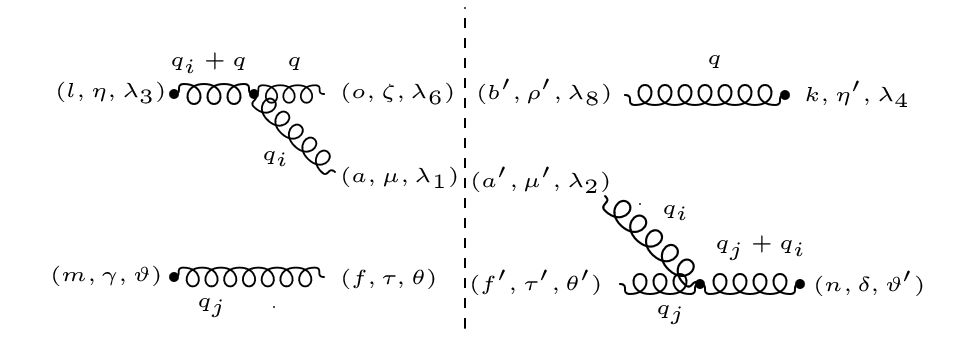
\includegraphics[width=0.95\textwidth]{images/GG/M1DaggerggInverse.png}
\end{figure}


\begin{equation}
\begin{split}
&M_1{M_2}^{\dagger}=\frac{g_s^2 f^{\:l\:o\:a} f^{\:f^{\prime}\: a^{\prime}\:n} \delta^{aa^{\prime}} \delta^{ob^{\prime}} \delta^{ff^{\prime}}}{(q_i +q)^2 (q_j +q_i)^2}
[{g_{{\zeta}}}^{{\eta}^{\prime}} {g^{\gamma}}_{{\tau}^{\prime}}(g^{{\eta}{\zeta}}(2q+q_i)^{\mu}+g^{{\zeta}{\mu}}(q_i -q)^{\eta}-g^{{\mu}{\eta}}(2q_i +q)^{\zeta})\\
&g_{{{\mu}}{{\mu}^{\prime}}}(g^{{{\tau}^{\prime}}{{\mu}^{\prime}}}(q_j-q_i)^{{\delta}}+g^{{{\mu}^{\prime}}{{\delta}}}(2q_i +q_j)^{{\tau}^{\prime}}-g^{{{\delta}}{{\tau}^{\prime}}}(2q_j+q_i)^{{\mu}^{\prime}}]
\end{split}
\end{equation}


\begin{equation}
\begin{split}
&M_1{M_2}^{\dagger}=\frac{g_s^2 f^{\:l\:o\:a} f^{\:f\: a\:n}}{4(q\cdot q_i) (q_i \cdot q_j)}\\
&[g^{{{\eta}}{{\eta}^{\prime}}}(2q+q_i)^{\gamma}(q_j-q_i)^{{\delta}}+g^{{{\eta}}{{\eta}^{\prime}}}(2q_i +q_j)^{\gamma}(2q+q_i)^{{\delta}}-g^{{{\eta}}{{\eta}^{\prime}}}g^{{{\gamma}}{{\delta}}}(2q+q_i)\cdot (2q_j+q_i)\\
&+g^{{{\gamma}}{{\eta}^{\prime}}}(q_i -q)^{\eta}(q_j+q_i)^{{\delta}}+g^{{{\eta}^{\prime}}{{\delta}}}(q_i -q)^{\eta}(2q_i +q_j)^{{\gamma}}
-g^{{{\gamma}}{{\delta}}}(q_i -q)^{\eta}(2q_j+q_i)^{{\eta}^{\prime}}\\
&-g^{{{\gamma}}{{\eta}}}(2q_i +q)^{{\eta}^{\prime}}(q_j-q_i)^{{\delta}}
-g^{{{\eta}}{{\delta}}}(2q_i +q)^{{\eta}^{\prime}}(2q_i +q_j)^{{\gamma}}
+g^{{{\gamma}}{{\delta}}}(2q_j+q_i)^{{\eta}}(2q_i +q)^{{\eta}^{\prime}}]\\
\end{split}
\end{equation}

\section*{Parametrization in terms of $ (k_1 \cdot q_i )(q_i \cdot q_k) $}
\begin{equation}
	\begin{aligned}
		\fbox{$  (k_1 \cdot q_i )(q_i \cdot q_k) {\color[RGB]{255,0,0} \: \approx\:} y\beta_1 (1-y)\:(p_i \cdot Q)(p_i \cdot p_k) $}
    \end{aligned}
\end{equation}

\subsection*{Calculation of the third term}

\begin{equation}
\begin{split}
&{\color[RGB]{255,0,0} -g^{{{\eta}}{{\eta}^{\prime}}}g^{{{\gamma}}{{\delta}}}}\lbrace 4{k_1}\cdot q_j+2k_1 \cdot q_i +2q_i \cdot q_k\rbrace
\end{split}
\end{equation}

\begin{equation}
\begin{split}
&M_1{M_2}^{\dagger}=\frac{g_s^2 C_A}{4y\beta_1 (1-y)\:(p_i \cdot p_k)(p_i \cdot Q)}
g^{{{\eta}}{{\eta}^{\prime}}}g^{{{\gamma}}{{\delta}}} \\
&[4([\alpha_1 (1-y)+y\beta_1(\frac{Q^2}{2p_i \cdot Q})]\:p_i \cdot p_k+y\beta_1\:Q\cdot p_k+\sqrt{\alpha_1\beta_1y(1-y)} p_k \cdot {n_{\bot,1}})\\
&2([\beta_1 (1-y)+y\alpha_1(\frac{Q^2}{2p_i \cdot Q})]\:p_i \cdot p_k+y\alpha_1\:Q\cdot p_k-\sqrt{\alpha_1\beta_1y(1-y)} p_k \cdot {n_{\bot,1}})\\
&+2(y\:p_i\cdot Q)]\\
\end{split}
\end{equation}

\begin{equation}
\begin{split}
&{\color[RGB]{255,0,0} -g^{{{\eta}}{{\eta}^{\prime}}}g^{{{\gamma}}{{\delta}}}}[ 4([\alpha_1 (1-y)+y\beta_1(\frac{Q^2}{2p_i \cdot Q})]\:p_i \cdot p_k+y\beta_1\:Q\cdot p_k+\sqrt{\alpha_1\beta_1y(1-y)} p_k \cdot {n_{\bot,1}})\\
&2([\beta_1 (1-y)+y\alpha_1(\frac{Q^2}{2p_i \cdot Q})]\:p_i \cdot p_k+y\alpha_1\:Q\cdot p_k-\sqrt{\alpha_1\beta_1y(1-y)} p_k \cdot {n_{\bot,1}})\\
&+2(y\:p_i\cdot Q)]
\end{split}
\end{equation}

\begin{equation}
\begin{split}
&M_1{M_2}^{\dagger}=g_s^2\: C_A\:g^{{{\eta}}{{\eta}^{\prime}}}g^{{{\gamma}}{{\delta}}}[\frac{1-\beta_1}{y\beta_1 (p_i \cdot Q)}+\frac{1}{2y(p_i \cdot Q)}+\frac{(1-\beta_1)(\frac{Q^2}{2p_i \cdot Q})}{2y\beta_1 (1-y)\:(p_i \cdot Q)}\\
&+\frac{(1-\beta_1)\:Q\cdot p_k}{2y\beta_1 (1-y)\:(p_i \cdot p_k)(p_i \cdot Q)}+\frac{1}{2(1-\beta_1)(1-y) (p_i \cdot p_k)}]\\
\end{split}
\end{equation}